\documentclass[letterpaper,12pt]{report}
\usepackage[utf8]{inputenc}
\usepackage[fleqn]{amsmath}
\usepackage{amsfonts}
\usepackage[x11names]{xcolor}
\usepackage{pgfplots}
\usepackage{tikz}

\usetikzlibrary{arrows.meta}
\pgfplotsset{
  compat = newest,
  blank_style/.style={
    clip=false,
    axis equal,
    axis line style={draw=none},
    tick style={draw=none},
    ticks=none,
    line width=1pt,
  },
  blank_clamped_style/.style={
    blank_style,
    xmin=-1,
    xmax=1,
    ymin=-0.25,
    ymax=1,
  },
}

\begin{document}

Let $P$ and $Q$ be two perpendicular lines in $\mathbb{R}^2$ and $\vec{x}$ a vector in $\mathbb{R}^2$. $Proj_P(\vec{x}) = \vec{u}$ and $Proj_Q(\vec{x}) = \vec{w}$. \\ \\
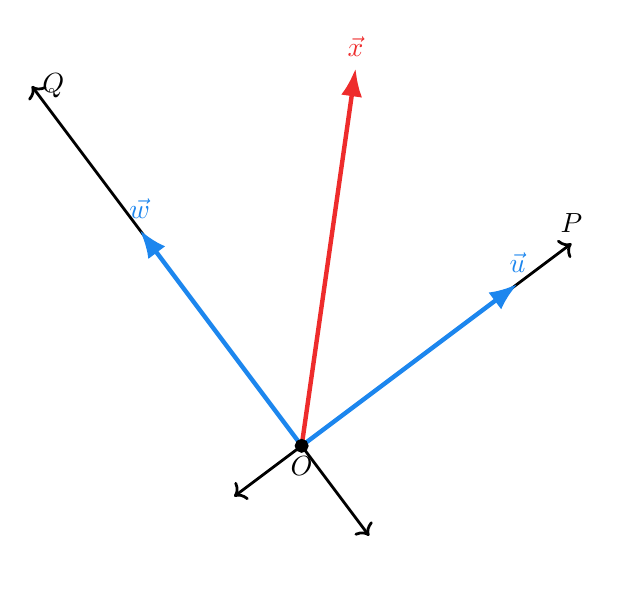
\begin{tikzpicture}
  \begin{axis}[blank_clamped_style]
    \addplot[<->, black, domain=-0.25:1]{3/4 * x} node[above,pos=1] {$P$};
    \addplot[<->, black, domain=-1:0.25]{-4/3 * x} node[right,pos=0] {$Q$};
    \addplot[black, mark=*] coordinates {(0, 0)} node[below,pos=1] {$O$};

    \addplot[-Latex, Firebrick2, ultra thick] coordinates {
      (0, 0)
      (1/5, 7/5)
    } node[above,pos=1] {$\vec{x}$};

    \addplot[-Latex, DodgerBlue2, ultra thick] coordinates {
      (0, 0)
      (4/5, 3/5)
    } node[above,pos=1] {$\vec{u}$};

    \addplot[-Latex, DodgerBlue2, ultra thick] coordinates {
      (0, 0)
      (-3/5, 4/5)
    } node[above,pos=1] {$\vec{w}$};
  \end{axis}
\end{tikzpicture} \\
To plot the vector sum $\vec{u} + \vec{w}$, place the vectors head to tail and then draw a vector from the free tail to the free head. \\ \\
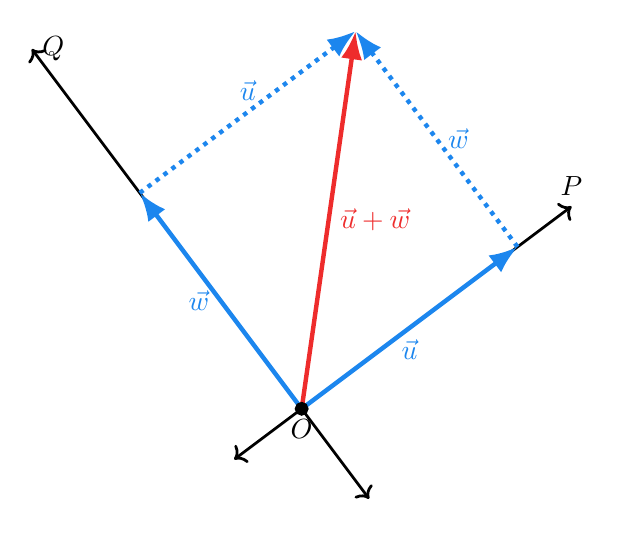
\begin{tikzpicture}
  \begin{axis}[blank_clamped_style]
    \addplot[<->, black, domain=-0.25:1]{3/4 * x} node[above,pos=1] {$P$};
    \addplot[<->, black, domain=-1:0.25]{-4/3 * x} node[right,pos=0] {$Q$};
    \addplot[black, mark=*] coordinates {(0, 0)} node[below,pos=1] {$O$};

    \addplot[-Latex, DodgerBlue2, ultra thick] coordinates {
      (0, 0)
      (4/5, 3/5)
    } node[below, midway] {$\vec{u}$};

    \addplot[-Latex, DodgerBlue2, ultra thick] coordinates {
      (0, 0)
      (-3/5, 4/5)
    } node[left, midway] {$\vec{w}$};

    \addplot[-Latex, DodgerBlue2, ultra thick, dotted] coordinates {
      (-3/5, 4/5)
      (1/5, 7/5)
    } node[above, midway] {$\vec{u}$};

    \addplot[-Latex, DodgerBlue2, ultra thick, dotted] coordinates {
      (4/5, 3/5)
      (1/5, 7/5)
    } node[right, midway] {$\vec{w}$};

    \addplot[-Latex, Firebrick2, ultra thick] coordinates {
      (0, 0)
      (1/5, 7/5)
    } node[right, midway] {$\vec{u} + \vec{w}$};
  \end{axis}
\end{tikzpicture} \\
Notice that $\vec{u} + \vec{w} = \vec{x}$. Therefore, $Proj_P(\vec{x}) + Proj_Q(\vec{x}) = \vec{x}$.

\end{document}
